\documentclass[10pt,a4paper]{article}

%double si on veut une version prof et une version élève. simple si on veut une seule version.
\newcommand{\buildmode}{simple}

\InputIfFileExists{version.tex}{}{}
% Version (définie par le script)
\providecommand{\version}{eleve}

\usepackage{feuillecorrection}

%%%à modifier à chaque fois

\renewcommand{\niveau}{1G}
\renewcommand{\chapitre}{Révisions}
\renewcommand{\numchap}{0 à 2}
\renewcommand{\theme}{Travail en distanciel}

%%% Arbre pondéré complété à deux niveaux
%%% #1 : évènement du 1er niveau ; #2 : évènement du 2nd niveau
%%% #3 = P(#1), #4 = P(non #1), #5 = P_#1(#2), #6 = P_#1(non #2),
%%% #7 = P_{non #1}(#2), #8 = P_{non #1}(non #2)
\newcommand{\arbre}[8]{
\begin{center}
\begin{tikzpicture}[
  grow'=right,
  level distance=3.2cm,
  level 1/.style={sibling distance=2.4cm},
  level 2/.style={sibling distance=1.9cm},
  edge from parent/.style={draw,-latex},
  every node/.style={font=\small}
]
\node {}
  child { node {\(#1\)}
    child { node {\(#2\)} edge from parent node[above] {\(#5\)} }
    child { node {\(\overline{#2}\)} edge from parent node[below] {\(#6\)} }
    edge from parent node[above] {\(#3\)}
  }
  child { node {\(\overline{#1}\)}
    child { node {\(#2\)} edge from parent node[above] {\(#7\)} }
    child { node {\(\overline{#2}\)} edge from parent node[below] {\(#8\)} }
    edge from parent node[below] {\(#4\)}
  };
\end{tikzpicture}
\end{center}
}

\begin{document}

\montitre{Révisions des premiers chapitres -- Correction}

%%%%%%%%%%%%%%%%%%%%%%%%%%%%%%%%%%%%%%%%%%%%%%%%%%%%%%%%%%%%%%%%%%%%%%%%%%%%%
\section{Fonctions affines et produits de fonctions affines}

\begin{corr}[Calculs de début de cours]{1}
\begin{enumerate}[leftmargin=*]
    \item Développements :
    \begin{tasks}[after-item-skip=0.3cm](2)
        \task \(3(2x-5)=6x-15\)
        \task \(\begin{aligned}[t] (x+2)(x-3)&=x^2-3x+2x-6\\ &=x^2-x-6\end{aligned}\)
        \task \(\begin{aligned}[t] (2x-1)(-x+4)&=-2x^2+8x+x-4\\ &=-2x^2+9x-4\end{aligned}\)
        \task \(\begin{aligned}[t] -(x-1)(x+5)&=-(x^2+5x-x-5)\\ &=-(x^2+4x-5)\\ &=-x^2-4x+5\end{aligned}\)
    \end{tasks}
    \item a) Identité. \quad b) Équation, de solution \(2\). \quad c) Identité. \quad d) Équation :

    \(\begin{aligned}[t] x^2+2x+1&=x^2+1\\ 2x+1&=1\\ 2x&=0\\ x&=0\end{aligned}\)

    L'égalité n'est vraie que pour \(x=0\) : ce n'est pas une identité.
\end{enumerate}
\end{corr}

\begin{corr}[Guidé]{2}
\begin{enumerate}[leftmargin=*]
    \item \(\begin{aligned}[t] 3x-2&=0\\ 3x&=2\\ x&=\dfrac{2}{3}\end{aligned}\)

    Le coefficient directeur \(3\) est positif : \(u\) est croissante, négative avant \(\dfrac{2}{3}\) et positive après.
    \item \(\begin{aligned}[t] -x+4&=0\\ -x&=-4\\ x&=4\end{aligned}\)

    Le coefficient directeur \(-1\) est négatif : \(v\) est décroissante, positive avant \(4\) et négative après.
    \item Tableau de signes :
    \begin{center}
    \begin{tikzpicture}
    \tkzTabInit[lgt=1.6,espcl=2]{\(x\) /1, \(3x-2\) /1, \(-x+4\) /1, \(f(x)\) /1}{\(-\infty\),\(\frac{2}{3}\),\(4\),\(+\infty\)}
    \tkzTabLine{,-,z,+,t,+,}
    \tkzTabLine{,+,t,+,z,-,}
    \tkzTabLine{,-,z,+,z,-,}
    \end{tikzpicture}
    \end{center}
    \item L'ensemble des solutions de \(f(x)\geq 0\) est \(\left[\dfrac{2}{3}\ ;\ 4\right]\).
    \item \(\begin{aligned}[t] f(0)&=(3\times 0-2)(-0+4)\\ &=(-2)\times 4\\ &=-8\end{aligned}\) \qquad \(\begin{aligned}[t] f(5)&=(3\times 5-2)(-5+4)\\ &=13\times(-1)\\ &=-13\end{aligned}\)

    Ces deux valeurs sont négatives, ce qui est cohérent avec le tableau : \(0\) et \(5\) sont en dehors de \(\left[\dfrac{2}{3}\ ;\ 4\right]\).
\end{enumerate}
\end{corr}

\begin{corr}{3}
\begin{enumerate}[leftmargin=*]
    \item \(f(0)=3\) et \(f(2)=-2\).
    \item Les antécédents de \(0\) sont \(-2\), \(1\) et \(3\).
    \item Tableau de signes :
    \begin{center}
    \begin{tikzpicture}
    \tkzTabInit[lgt=1.1,espcl=1.6]{\(x\) /1, \(f(x)\) /1}{{\(-2{,}5\)},\(-2\),\(1\),\(3\),{\(3{,}5\)}}
    \tkzTabLine{,-,z,+,z,-,z,+,}
    \end{tikzpicture}
    \end{center}
    \item \(f(x)\geq 0\) pour \(x\in[-2\ ;\ 1]\cup[3\ ;\ 3,5]\).
    \item \(\begin{aligned}[t] f(0)&=0,5\times 2\times(-1)\times(-3)\\ &=3\end{aligned}\) \qquad \(\begin{aligned}[t] f(2)&=0,5\times 4\times 1\times(-1)\\ &=-2\end{aligned}\)

    On retrouve les lectures graphiques de la question 1.
\end{enumerate}
\end{corr}

\begin{corr}{4}
Exemple de rédaction complète pour \(g\) :

\textit{Méthode 1 (par le calcul).}
\[
\begin{aligned}
-4x+2 &\geq 0\\
-4x+2\textcolor{teal}{-2} &\geq 0\textcolor{teal}{-2}\\
-4x &\geq -2\\
-4x\textcolor{teal}{\div(-4)} &\leq -2\textcolor{teal}{\div(-4)}\\
x &\leq \frac{1}{2}
\end{aligned}
\]
(on divise par \(-4<0\) : l'inégalité change de sens).

\textit{Méthode 2 (graphique).} \(a=-4<0\) : la droite descend et coupe l'axe des abscisses en \(\dfrac{1}{2}\).

\medskip

Tableaux de signes :
\begin{enumerate}[label=\alph*)]
    \item \(f(x)=3x-6\) : \(a=3>0\), donc \(f\) est croissante. On résout \(3x-6=0\) :

    \(\begin{aligned}[t] 3x-6&=0\\ 3x&=6\\ x&=2\end{aligned}\)
    \begin{center}
    \begin{tikzpicture}
    \tkzTabInit[lgt=1.1,espcl=1.6]{\(x\) /1, \(f(x)\) /1}{\(-\infty\),\(2\),\(+\infty\)}
    \tkzTabLine{,-,z,+,}
    \end{tikzpicture}
    \end{center}
    \item \(g(x)=-4x+2\) : \(a=-4<0\), donc \(g\) est décroissante. On résout \(-4x+2=0\) :

    \(\begin{aligned}[t] -4x+2&=0\\ -4x&=-2\\ x&=\dfrac{-2}{-4}\\ x&=\dfrac{1}{2}\end{aligned}\)
    \begin{center}
    \begin{tikzpicture}
    \tkzTabInit[lgt=1.1,espcl=1.6]{\(x\) /1, \(g(x)\) /1}{\(-\infty\),\(\frac{1}{2}\),\(+\infty\)}
    \tkzTabLine{,+,z,-,}
    \end{tikzpicture}
    \end{center}
    \item \(h(x)=x+5\) : \(a=1>0\), donc \(h\) est croissante. On résout \(x+5=0\) :

    \(\begin{aligned}[t] x+5&=0\\ x&=-5\end{aligned}\)
    \begin{center}
    \begin{tikzpicture}
    \tkzTabInit[lgt=1.1,espcl=1.6]{\(x\) /1, \(h(x)\) /1}{\(-\infty\),\(-5\),\(+\infty\)}
    \tkzTabLine{,-,z,+,}
    \end{tikzpicture}
    \end{center}
    \item \(k(x)=-x-3\) : \(a=-1<0\), donc \(k\) est décroissante. On résout \(-x-3=0\) :

    \(\begin{aligned}[t] -x-3&=0\\ -x&=3\\ x&=-3\end{aligned}\)
    \begin{center}
    \begin{tikzpicture}
    \tkzTabInit[lgt=1.1,espcl=1.6]{\(x\) /1, \(k(x)\) /1}{\(-\infty\),\(-3\),\(+\infty\)}
    \tkzTabLine{,+,z,-,}
    \end{tikzpicture}
    \end{center}
\end{enumerate}
\end{corr}

\begin{corr}{5}
\begin{enumerate}[leftmargin=*]
    \item \(\begin{aligned}[t] x+2&=0\\ x&=-2\end{aligned}\) \qquad \(\begin{aligned}[t] 2x-5&=0\\ 2x&=5\\ x&=\dfrac{5}{2}\end{aligned}\)
    \begin{center}
    \begin{tikzpicture}
    \tkzTabInit[lgt=1.6,espcl=2]{\(x\) /1, \(x+2\) /1, \(2x-5\) /1, \(f(x)\) /1}{\(-\infty\),\(-2\),\(\frac{5}{2}\),\(+\infty\)}
    \tkzTabLine{,-,z,+,t,+,}
    \tkzTabLine{,-,t,-,z,+,}
    \tkzTabLine{,+,z,-,z,+,}
    \end{tikzpicture}
    \end{center}
    \(f(x)<0\) pour \(x\in\left]-2\ ;\ \dfrac{5}{2}\right[\).
    \item \(\begin{aligned}[t] -3x+1&=0\\ -3x&=-1\\ x&=\dfrac{1}{3}\end{aligned}\) \qquad \(\begin{aligned}[t] x+4&=0\\ x&=-4\end{aligned}\)
    \begin{center}
    \begin{tikzpicture}
    \tkzTabInit[lgt=1.6,espcl=2]{\(x\) /1, \(-3x+1\) /1, \(x+4\) /1, \(g(x)\) /1}{\(-\infty\),\(-4\),\(\frac{1}{3}\),\(+\infty\)}
    \tkzTabLine{,+,t,+,z,-,}
    \tkzTabLine{,-,z,+,t,+,}
    \tkzTabLine{,-,z,+,z,-,}
    \end{tikzpicture}
    \end{center}
    \(g(x)\geq 0\) pour \(x\in\left[-4\ ;\ \dfrac{1}{3}\right]\).
    \item Le facteur \(x\) s'annule en \(0\).

    \(\begin{aligned}[t] 4-x&=0\\ -x&=-4\\ x&=4\end{aligned}\)
    \begin{center}
    \begin{tikzpicture}
    \tkzTabInit[lgt=1.6,espcl=2]{\(x\) /1, \(x\) /1, \(4-x\) /1, \(h(x)\) /1}{\(-\infty\),\(0\),\(4\),\(+\infty\)}
    \tkzTabLine{,-,z,+,t,+,}
    \tkzTabLine{,+,t,+,z,-,}
    \tkzTabLine{,-,z,+,z,-,}
    \end{tikzpicture}
    \end{center}
    \(h(x)>0\) pour \(x\in\,]0\ ;\ 4[\).
\end{enumerate}
\end{corr}

\begin{corr}{6}
\begin{enumerate}[leftmargin=*]
    \item \(f(x)\) n'est ni une expression affine, ni un produit de fonctions affines : les méthodes de cette section ne s'appliquent pas directement.
    \item \(\begin{aligned}[t] (2x+1)(x-2)&=2x^2-4x+x-2\\ &=2x^2-3x-2\end{aligned}\)

    On a montré que \((2x+1)(x-2)=2x^2-3x-2\) ; or \(f(x)=2x^2-3x-2\) ; donc \(f(x)=(2x+1)(x-2)\) pour tout réel \(x\).
    \item \(\begin{aligned}[t] 2x+1&=0\\ 2x&=-1\\ x&=-\dfrac{1}{2}\end{aligned}\) \qquad \(\begin{aligned}[t] x-2&=0\\ x&=2\end{aligned}\)
    \begin{center}
    \begin{tikzpicture}
    \tkzTabInit[lgt=1.6,espcl=2]{\(x\) /1, \(2x+1\) /1, \(x-2\) /1, \(f(x)\) /1}{\(-\infty\),\(-\frac{1}{2}\),\(2\),\(+\infty\)}
    \tkzTabLine{,-,z,+,t,+,}
    \tkzTabLine{,-,t,-,z,+,}
    \tkzTabLine{,+,z,-,z,+,}
    \end{tikzpicture}
    \end{center}
    \(f(x)<0\) pour \(x\in\left]-\dfrac{1}{2}\ ;\ 2\right[\).
\end{enumerate}
\end{corr}

%%%%%%%%%%%%%%%%%%%%%%%%%%%%%%%%%%%%%%%%%%%%%%%%%%%%%%%%%%%%%%%%%%%%%%%%%%%%%
\section{Suites, généralités}

\begin{corr}[Calculs de début de cours]{7}
\begin{enumerate}[leftmargin=*]
    \item Un produit est nul si et seulement si l'un de ses facteurs est nul.
    \begin{tasks}(3)
        \task \(\begin{aligned}[t] x-3&=0 &\text{ou}\quad 2x+5&=0\\ x&=3 & 2x&=-5\\ & & x&=-\dfrac{5}{2}\end{aligned}\)
        \task \(\begin{aligned}[t] x&=0 &\text{ou}\quad x+7&=0\\ & & x&=-7\end{aligned}\)
        \task \(\begin{aligned}[t] 4-x&=0 &\text{ou}\quad 3x-1&=0\\ -x&=-4 & 3x&=1\\ x&=4 & x&=\dfrac{1}{3}\end{aligned}\)
    \end{tasks}
    \item Pour \(n\) entier naturel (\(n\geq 0\)) :
    \begin{tasks}(2)
        \task \(2n+3\geq 3>0\) : positif
        \task \(-5<0\) : négatif
        \task \(n^2+1\geq 1>0\) : positif
        \task \(-2n-1\leq -1<0\) : négatif
    \end{tasks}
\end{enumerate}
\end{corr}

\begin{corr}[Guidé]{8}
\begin{enumerate}[leftmargin=*]
    \item \begin{tasks}[after-item-skip=0.2cm](3)
        \task \(u_0=3\)
        \task \(\begin{aligned}[t] u_1&=1-4+3\\ &=0\end{aligned}\)
        \task \(\begin{aligned}[t] u_2&=4-8+3\\ &=-1\end{aligned}\)
        \task \(\begin{aligned}[t] u_3&=9-12+3\\ &=0\end{aligned}\)
        \task \(\begin{aligned}[t] u_4&=16-16+3\\ &=3\end{aligned}\)
        \task \(\begin{aligned}[t] u_5&=25-20+3\\ &=8\end{aligned}\)
    \end{tasks}
    \item Nuage de points :
    \begin{center}
    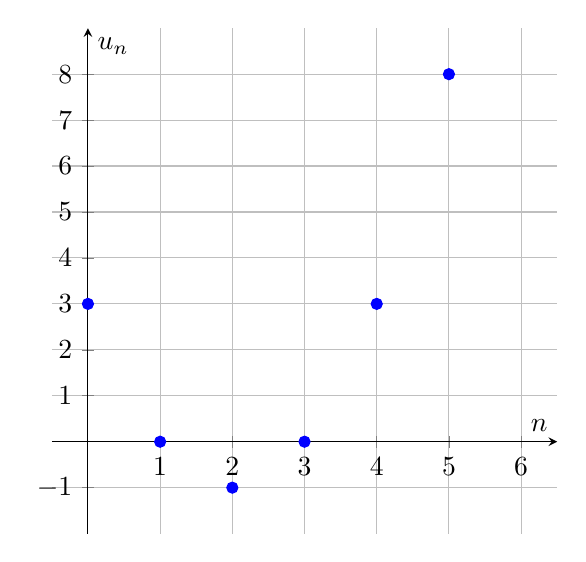
\begin{tikzpicture}
    \begin{axis}[
        axis lines=middle,
        xmin=-0.5, xmax=6.5,
        ymin=-2, ymax=9,
        grid=major,
        xtick={0,1,...,6},
        ytick={-1,0,...,8},
        xlabel={\(n\)},
        ylabel={\(u_n\)},
        width=8cm,
        height=8cm
    ]
    \addplot[only marks, mark=*, mark size=2pt, blue] coordinates {(0,3)(1,0)(2,-1)(3,0)(4,3)(5,8)};
    \end{axis}
    \end{tikzpicture}
    \end{center}
    \item À partir du rang \(2\), la suite semble croissante.
    \item \(\begin{aligned}[t] u_{n+1}&=(n+1)^2-4(n+1)+3\\ &=n^2+2n+1-4n-4+3\\ &=n^2-2n\end{aligned}\)
    \item \(\begin{aligned}[t] u_{n+1}-u_n&=(n^2-2n)-(n^2-4n+3)\\ &=n^2-2n-n^2+4n-3\\ &=2n-3\end{aligned}\)
    \item \(\begin{aligned}[t] 2n-3&\geq 0\\ 2n&\geq 3\\ n&\geq \dfrac{3}{2}\end{aligned}\)

    Pour un entier naturel, cela signifie \(n\geq 2\). Ainsi, pour tout \(n\geq 2\), \(u_{n+1}-u_n\geq 0\) : la suite est croissante à partir du rang \(2\). Elle n'est pas croissante dès le départ, puisque \(u_1-u_0=-3<0\).
\end{enumerate}
\end{corr}

\begin{corr}{9}
\begin{enumerate}[leftmargin=*]
    \item \(u_1=2\) ; \(u_2=11\) ; \(u_4=47\). Définition explicite : \(u_n\) est donné directement en fonction de \(n\).
    \item \(u_1=\dfrac{2}{3}\) ; \(u_2=\dfrac{3}{4}\) ; \(u_4=\dfrac{5}{6}\). Définition explicite.
    \item \(\begin{aligned}[t] u_1&=-2\times(-2)+1\\ &=5\end{aligned}\) \qquad \(\begin{aligned}[t] u_2&=-2\times 5+1\\ &=-9\end{aligned}\) \qquad \(\begin{aligned}[t] u_3&=-2\times(-9)+1\\ &=19\end{aligned}\) \qquad \(\begin{aligned}[t] u_4&=-2\times 19+1\\ &=-37\end{aligned}\)

    Définition par récurrence.
    \item[\(\star\)~4.] \(\begin{aligned}[t] u_1&=u_0+2\times 0\\ &=1\end{aligned}\) \qquad \(\begin{aligned}[t] u_2&=u_1+2\times 1\\ &=3\end{aligned}\) \qquad \(\begin{aligned}[t] u_3&=u_2+2\times 2\\ &=7\end{aligned}\) \qquad \(\begin{aligned}[t] u_4&=u_3+2\times 3\\ &=13\end{aligned}\)

    Définition par récurrence : chaque terme se calcule à partir du précédent, il faut donc calculer \(u_3\) pour obtenir \(u_4\).
\end{enumerate}
Pour la suite 1 :

\(\begin{aligned}[t] u_{n+1}&=3(n+1)^2-1\\ &=3(n^2+2n+1)-1\\ &=3n^2+6n+2\end{aligned}\)
\end{corr}

\begin{corr}{10}
\begin{tasks}[after-item-skip=0.2cm](1)
    \task \(\begin{aligned}[t] u_{n+1}-u_n&=5(n+1)-2-(5n-2)\\ &=5n+5-2-5n+2\\ &=5\end{aligned}\)

    \(5>0\) : la suite est croissante.
    \task \(\begin{aligned}[t] u_{n+1}-u_n&=-3(n+1)+7-(-3n+7)\\ &=-3n-3+7+3n-7\\ &=-3\end{aligned}\)

    \(-3<0\) : la suite est décroissante.
    \task \(\begin{aligned}[t] u_{n+1}-u_n&=(n+1)^2+2(n+1)-(n^2+2n)\\ &=n^2+2n+1+2n+2-n^2-2n\\ &=2n+3\end{aligned}\)

    Pour tout entier naturel \(n\), \(2n+3>0\) : la suite est croissante.
    \task \(\begin{aligned}[t] u_{n+1}-u_n&=\dfrac{1}{n+3}-\dfrac{1}{n+2}\\ &=\dfrac{(n+2)-(n+3)}{(n+2)(n+3)}\\ &=\dfrac{-1}{(n+2)(n+3)}\end{aligned}\)

    Pour tout entier naturel \(n\), le dénominateur est positif, donc \(u_{n+1}-u_n<0\) : la suite est décroissante.
    \task \(u_{n+1}-u_n=-n^2-1<0\) (voir les calculs de début de cours) : la suite est décroissante.
\end{tasks}
\end{corr}

\begin{corr}{11}
\begin{enumerate}[leftmargin=*]
    \item On ajoute \(3\) à chaque étape. Définition explicite : \(u_n=3n+2\). Définition par récurrence : \(u_0=2\) et \(u_{n+1}=u_n+3\).
    \item \begin{enumerate}
        \item Vrai : pour tout \(n\), \(u_{n+1}-u_n=3>0\), donc la suite est croissante.
        \item Faux. Contre-exemple : la suite 4 de l'exercice 9 vérifie \(u_0<u_1\) (\(u_0=-2\) et \(u_1=5\)), mais \(u_2<u_1\) (\(u_2=-9\)) : elle n'est pas croissante.
    \end{enumerate}
\end{enumerate}
\end{corr}

%%%%%%%%%%%%%%%%%%%%%%%%%%%%%%%%%%%%%%%%%%%%%%%%%%%%%%%%%%%%%%%%%%%%%%%%%%%%%
\section{Probabilités conditionnelles}

\begin{corr}[Calculs de début de cours]{12}
\begin{enumerate}[leftmargin=*]
    \item Tableau complété :
    \begin{center}
    \renewcommand{\arraystretch}{1.8}
    \begin{tabular}{|c|c|c|c|c|c|}
        \hline
        Fraction irréductible & \(\dfrac{3}{4}\) & \(\dfrac{2}{5}\) & \(\dfrac{3}{20}\) & \(\dfrac{1}{8}\) & \(\dfrac{7}{20}\) \\ \hline
        Décimal & \(0,75\) & \(0,4\) & \(0,15\) & \(0,125\) & \(0,35\) \\ \hline
        Pourcentage & \(75\,\%\) & \(40\,\%\) & \(15\,\%\) & \(12,5\,\%\) & \(35\,\%\) \\ \hline
    \end{tabular}
    \end{center}
    \item \(A\cap B=\{2;4\}\) ; \(A\cup B=\{1;2;3;4;6;8;10\}\) ; \(\overline{A}=\{1;3;5;7;9\}\).
\end{enumerate}
\end{corr}

\begin{corr}[Guidé]{13}
\begin{enumerate}[leftmargin=*]
    \item \(\begin{aligned}[t] P(M)&=\dfrac{90}{250}\\ &=0,36\end{aligned}\)
    \item \(M\cap B\) : \og l'usager est mineur et emprunte des BD \fg{}.

    \(\begin{aligned}[t] P(M\cap B)&=\dfrac{60}{250}\\ &=0,24\end{aligned}\)
    \item \(\begin{aligned}[t] P_M(B)&=\dfrac{60}{90}\\ &=\dfrac{2}{3}\\ &\approx 0,667\end{aligned}\)

    Parmi les usagers mineurs, environ \(66,7\,\%\) empruntent des BD.
    \item \(\begin{aligned}[t] P_B(M)&=\dfrac{60}{100}\\ &=0,6\end{aligned}\)

    Parmi les emprunteurs de BD, \(60\,\%\) sont mineurs. On a \(P_M(B)\neq P_B(M)\) : on ne se restreint pas à la même sous-population.
    \item \(\begin{aligned}[t] \dfrac{P(M\cap B)}{P(M)}&=\dfrac{0,24}{0,36}\\ &=\dfrac{24}{36}\\ &=\dfrac{2}{3}\end{aligned}\)

    On retrouve bien \(P_M(B)\).
\end{enumerate}
\end{corr}

\begin{corr}{14}
\begin{enumerate}[leftmargin=*]
    \item Arbre pondéré :
    \arbre{P}{S}{0,4}{0,6}{0,75}{0,25}{0,5}{0,5}
    \item \(P_P(S)=0,75\).
    \item \(\begin{aligned}[t] P(P\cap S)&=0,4\times 0,75\\ &=0,3\end{aligned}\) \qquad \(\begin{aligned}[t] P(P\cap\overline{S})&=0,4\times 0,25\\ &=0,1\end{aligned}\)

    \(10\,\%\) des abonnés ont l'offre Premium et ne regardent pas de séries chaque semaine.
    \item \(\begin{aligned}[t] P(\overline{P}\cap\overline{S})&=0,6\times 0,5\\ &=0,3\end{aligned}\)
    \item \(P_P(S)\) se lit directement sur l'arbre. \(P(P\cap S)\) se calcule avec la règle du produit. \(P_S(P)\) ne peut être obtenue ni par lecture ni par la règle du produit : il faudrait connaître \(P(S)\).
\end{enumerate}
\end{corr}

\begin{corr}{15}
\begin{enumerate}[leftmargin=*]
    \item \(\begin{aligned}[t] P(L)&=\dfrac{60}{200}\\ &=0,3\end{aligned}\) \qquad \(\begin{aligned}[t] P_L(T)&=\dfrac{45}{60}\\ &=0,75\end{aligned}\) \qquad \(\begin{aligned}[t] P_{\overline{L}}(T)&=\dfrac{35}{140}\\ &=0,25\end{aligned}\)
    \arbre{L}{T}{0,3}{0,7}{0,75}{0,25}{0,25}{0,75}
    \item Avec l'arbre : \(\begin{aligned}[t] P(L\cap T)&=0,3\times 0,75\\ &=0,225\end{aligned}\) \qquad Avec le tableau : \(\begin{aligned}[t] P(L\cap T)&=\dfrac{45}{200}\\ &=0,225\end{aligned}\)

    Les deux résultats sont égaux.
    \item \(\begin{aligned}[t] P_T(L)&=\dfrac{45}{80}\\ &=0,5625\end{aligned}\)

    Parmi les salariés en télétravail, \(56,25\,\%\) ont un trajet de plus d'une heure.
\end{enumerate}
\end{corr}

\begin{corr}{16}
\begin{enumerate}[leftmargin=*]
    \item \begin{enumerate}
        \item Arbre pondéré :
        \arbre{A}{B}{x}{1-x}{0,6}{0,4}{0,2}{0,8}
        \item \(\begin{aligned}[t] P(A\cap B)&=P(A)\times P_A(B)\\ &=0,6x\end{aligned}\)

        Comme \(P(A\cap B)=0,24\) :

        \(\begin{aligned}[t] 0,6x&=0,24\\ x&=\dfrac{0,24}{0,6}\\ x&=0,4\end{aligned}\)
        \item \(\begin{aligned}[t] P(\overline{A}\cap B)&=(1-0,4)\times 0,2\\ &=0,6\times 0,2\\ &=0,12\end{aligned}\)
    \end{enumerate}
    \item \(P_C(\overline{D})=1-y\), donc \(P(C\cap\overline{D})=0,3(1-y)\). Comme \(P(C\cap\overline{D})=0,12\) :

    \(\begin{aligned}[t] 0,3(1-y)&=0,12\\ 1-y&=\dfrac{0,12}{0,3}\\ 1-y&=0,4\\ -y&=-0,6\\ y&=0,6\end{aligned}\)
\end{enumerate}
\end{corr}

%%%%%%%%%%%%%%%%%%%%%%%%%%%%%%%%%%%%%%%%%%%%%%%%%%%%%%%%%%%%%%%%%%%%%%%%%%%%%
\section{Problèmes}

\begin{corr}[Abonnés d'une plateforme]{17}
\begin{enumerate}[leftmargin=*]
    \item \(\begin{aligned}[t] a_1&=2\,000-200+300\\ &=2\,100\end{aligned}\) \qquad \(\begin{aligned}[t] a_2&=2\,100-210+300\\ &=2\,190\end{aligned}\)
    \item Perdre \(10\,\%\) des abonnés revient à multiplier par \(0,9\), puis on ajoute les \(300\) nouveaux abonnés : \(a_{n+1}=0,9\,a_n+300\). La suite est définie par récurrence (avec \(a_0=2\,000\)).
    \item \(\begin{aligned}[t] a_3&=0,9\times 2\,190+300\\ &=2\,271\end{aligned}\) \qquad \(\begin{aligned}[t] a_4&=0,9\times 2\,271+300\\ &=2\,343,9\\ &\approx 2\,344\end{aligned}\)

    La suite semble croissante.
    \item \begin{enumerate}
        \item \(\begin{aligned}[t] a_0&=3\,000-1\,000\times 0,9^0\\ &=3\,000-1\,000\\ &=2\,000\end{aligned}\) \qquad \(\begin{aligned}[t] a_1&=3\,000-1\,000\times 0,9\\ &=3\,000-900\\ &=2\,100\end{aligned}\)

        On retrouve les valeurs de la question 1 : la formule est cohérente.
        \item \(\begin{aligned}[t] a_{n+1}-a_n&=\left(3\,000-1\,000\times 0,9^{n+1}\right)-\left(3\,000-1\,000\times 0,9^n\right)\\ &=1\,000\times 0,9^n-1\,000\times 0,9^{n+1}\\ &=1\,000\times 0,9^n-1\,000\times 0,9\times 0,9^n\\ &=1\,000\times 0,9^n-900\times 0,9^n\\ &=100\times 0,9^n\end{aligned}\)
        \item Pour tout \(n\), \(0,9^n>0\), donc \(a_{n+1}-a_n>0\) : la suite \((a_n)\) est croissante.
    \end{enumerate}
\end{enumerate}
\end{corr}

\begin{corr}[Une petite entreprise]{18}
\begin{enumerate}[leftmargin=*]
    \item \(\begin{aligned}[t] B(0)&=(0-2)(-3\times 0+30)\\ &=(-2)\times 30\\ &=-60\end{aligned}\)

    Sans production, l'entreprise perd \(60\,000\) euros par semaine.
    \item \(\begin{aligned}[t] x-2&=0\\ x&=2\end{aligned}\) \qquad \(\begin{aligned}[t] -3x+30&=0\\ -3x&=-30\\ x&=10\end{aligned}\)
    \begin{center}
    \begin{tikzpicture}
    \tkzTabInit[lgt=1.8,espcl=2]{\(x\) /1, \(x-2\) /1, \(-3x+30\) /1, \(B(x)\) /1}{\(0\),\(2\),\(10\),\(12\)}
    \tkzTabLine{,-,z,+,t,+,}
    \tkzTabLine{,+,t,+,z,-,}
    \tkzTabLine{,-,z,+,z,-,}
    \end{tikzpicture}
    \end{center}
    \item \(B(x)>0\) pour \(x\in\,]2\ ;\ 10[\) : l'entreprise réalise un bénéfice lorsqu'elle fabrique entre \(200\) et \(1\,000\) objets par semaine.
    \item \begin{enumerate}
        \item Arbre pondéré :
        \arbre{A}{D}{0,7}{0,3}{0,02}{0,98}{0,05}{0,95}
        \item \(\begin{aligned}[t] P(A\cap D)&=0,7\times 0,02\\ &=0,014\end{aligned}\) \qquad \(\begin{aligned}[t] P(\overline{A}\cap D)&=0,3\times 0,05\\ &=0,015\end{aligned}\)
        \item L'affirmation est fausse : \(0,015>0,014\). Bien qu'elle fabrique moins d'objets, la chaîne \(\overline{A}\) fournit un peu plus d'objets défectueux, car sa proportion de défauts est plus forte.
    \end{enumerate}
\end{enumerate}
\end{corr}

\end{document}
